%----------------------------------------------------------------------------
%
% 
% 
%
%----------------------------------------------------------------------------
%----------------------------------------------------------------------------
%----------------------------------------------------------------------------

\ProvidesFile{proposal.tex}
\documentclass[cameraready]{acmsiggraph-awb}
\usepackage[scaled=.92]{helvet}
\usepackage{times}
\usepackage{algorithm}
\usepackage{algorithmic}

\usepackage[pdftex]{graphicx} \pdfcompresslevel=9

\usepackage{parskip}

\usepackage[labelfont=bf,textfont=it]{caption}

\usepackage{amsmath}
\usepackage{amssymb}
\usepackage{wasysym}
\usepackage{bm}
\usepackage{cite}
\usepackage{enumerate}

\usepackage{url}

% For backwards compatibility to old LaTeX type font selection.
% Uncomment if your document adheres to LaTeX2e recommendations.
\let\rm=\rmfamily    \let\sf=\sffamily    \let\tt=\ttfamily
\let\it=\itshape     \let\sl=\slshape     \let\sc=\scshape
\let\bf=\bfseries

% end of prologue
\usepackage[%
 breaklinks,
 letterpaper,
 bookmarks,
 bookmarksnumbered,
 colorlinks,
 linkcolor={black},
 citecolor={black},
 pdfpagemode={None},
]{hyperref}
\setlength\paperwidth{8.5in}  % Override any random settings...
\setlength\paperheight{11in}

\DeclareMathOperator*{\argmin}{\arg\!\min}


\newcommand{\etal}{et al.}
\newcommand{\hidecomment}[1]{}
\newcommand{\Mueller}{M\"{u}ller\ }
\newcommand{\Bez}{B\'{e}zier\ }
\newcommand{\BM}[1]{\B{#1}}
%\newcommand{\B}[1]{\mbox{\boldmath$#1$}}
%\newcommand{\B}[1]{\textbf{\textit{#1}}}
\newcommand{\B}[1]{\mathit{\mathbf{#1}}}
%\newcommand{\B}[1]{\boldsymbol{#1}}
\newcommand{\Per}{\%}
\newcommand{\Unit}[1]{{\mbox{$\,\mathrm{#1}$}}}
\newcommand{\Snit}[1]{{\mbox{\small$\mathrm{#1}$}}}
\newcommand{\Tr}[1]{\mathrm{Tr}\left(#1\right)}
\newcommand{\Hz}{\Unit{Hz}}
\newcommand{\MHz}{\Unit{MHz}}
\newcommand{\GHz}{\Unit{GHz}}
\newcommand{\Sec}{\Unit{sec}}
\newcommand{\SPF}{\Unit{sec/frame}}
\newcommand{\Min}{\Unit{min}}
\newcommand{\Max}{\Unit{max}}
\newcommand{\M}{\Unit{m}}
\newcommand{\Nab}{\B{\nabla}}
\newcommand{\TP}{^\mathsf{T}}

\newcommand{\Dist}{\mbox{dist}}

\newcommand{\figureTopBot}[1]{
  \begin{figure}[!tb]{\sloppy #1}\end{figure}
}

\newcommand{\figureTop}[1]{
  \begin{figure}[!t]{\sloppy #1}\end{figure}
}
 
\newcommand{\figureBot}[1]{
  \begin{figure}[!b]{\sloppy #1}\end{figure}
}

\newcommand{\figureWideTop}[1]{
  \begin{figure*}[!t]{\sloppy #1}\end{figure*}
}

\newcommand{\eqAlgn}{\!\!&\!\!}

\newcommand{\Eref}[1]{Equation~(\ref{#1})}
\newcommand{\Erefs}[2]{Equations~(\ref{#1}) and (\ref{#2})}
\newcommand{\eref}[1]{Equation~(\ref{#1})}
\newcommand{\erefs}[2]{Equations~(\ref{#1}) and (\ref{#2})}
\newcommand{\Sref}[1]{Section~\ref{#1}}
\newcommand{\sref}[1]{Section~\ref{#1}}
\newcommand{\fref}[1]{Figure~\ref{#1}}
\newcommand{\frefAND}[2]{Figures~\ref{#1} and~\ref{#2}}
\newcommand{\frefs}[2]{Figures~\ref{#1} and~\ref{#2}}
\newcommand{\frefss}[3]{Figures~\ref{#1}, \ref{#2}, and~\ref{#3}}
\newcommand{\Fref}[1]{Figure~\ref{#1}}
\newcommand{\Frefs}[2]{Figures~\ref{#1} and~\ref{#2}}
\newcommand{\Frefss}[3]{Figures~\ref{#1}, \ref{#2}, and~\ref{#3}}
\newcommand{\tref}[1]{Table~\ref{#1}}

\renewcommand{\labelenumi}{\arabic{enumi}.}
\renewcommand{\labelenumii}{\alph{enumii}.}
\renewcommand{\labelenumiii}{\roman{enumiii}.}

\newenvironment{algstep}{%
  \begin{enumerate}%
    \setlength{\itemsep}{0in}%
    \setlength{\partopsep}{0in}%
    \setlength{\topsep}{0in}%
}{\end{enumerate}}





\onlineid{papers\_0632}
\newcommand{\theTitle}{GPU Accelerated Point-Based Elastoplastic Solid Simulation}

\title{\theTitle}

\author{
	Ben Jones \and Kyle Hansen}

\newcommand{\theKeywords}{%
  viscoelastic materials, point-based animation, natural phenomena, physics-based animation.%
}


\begin{document}

\teaser{\begin{centering}
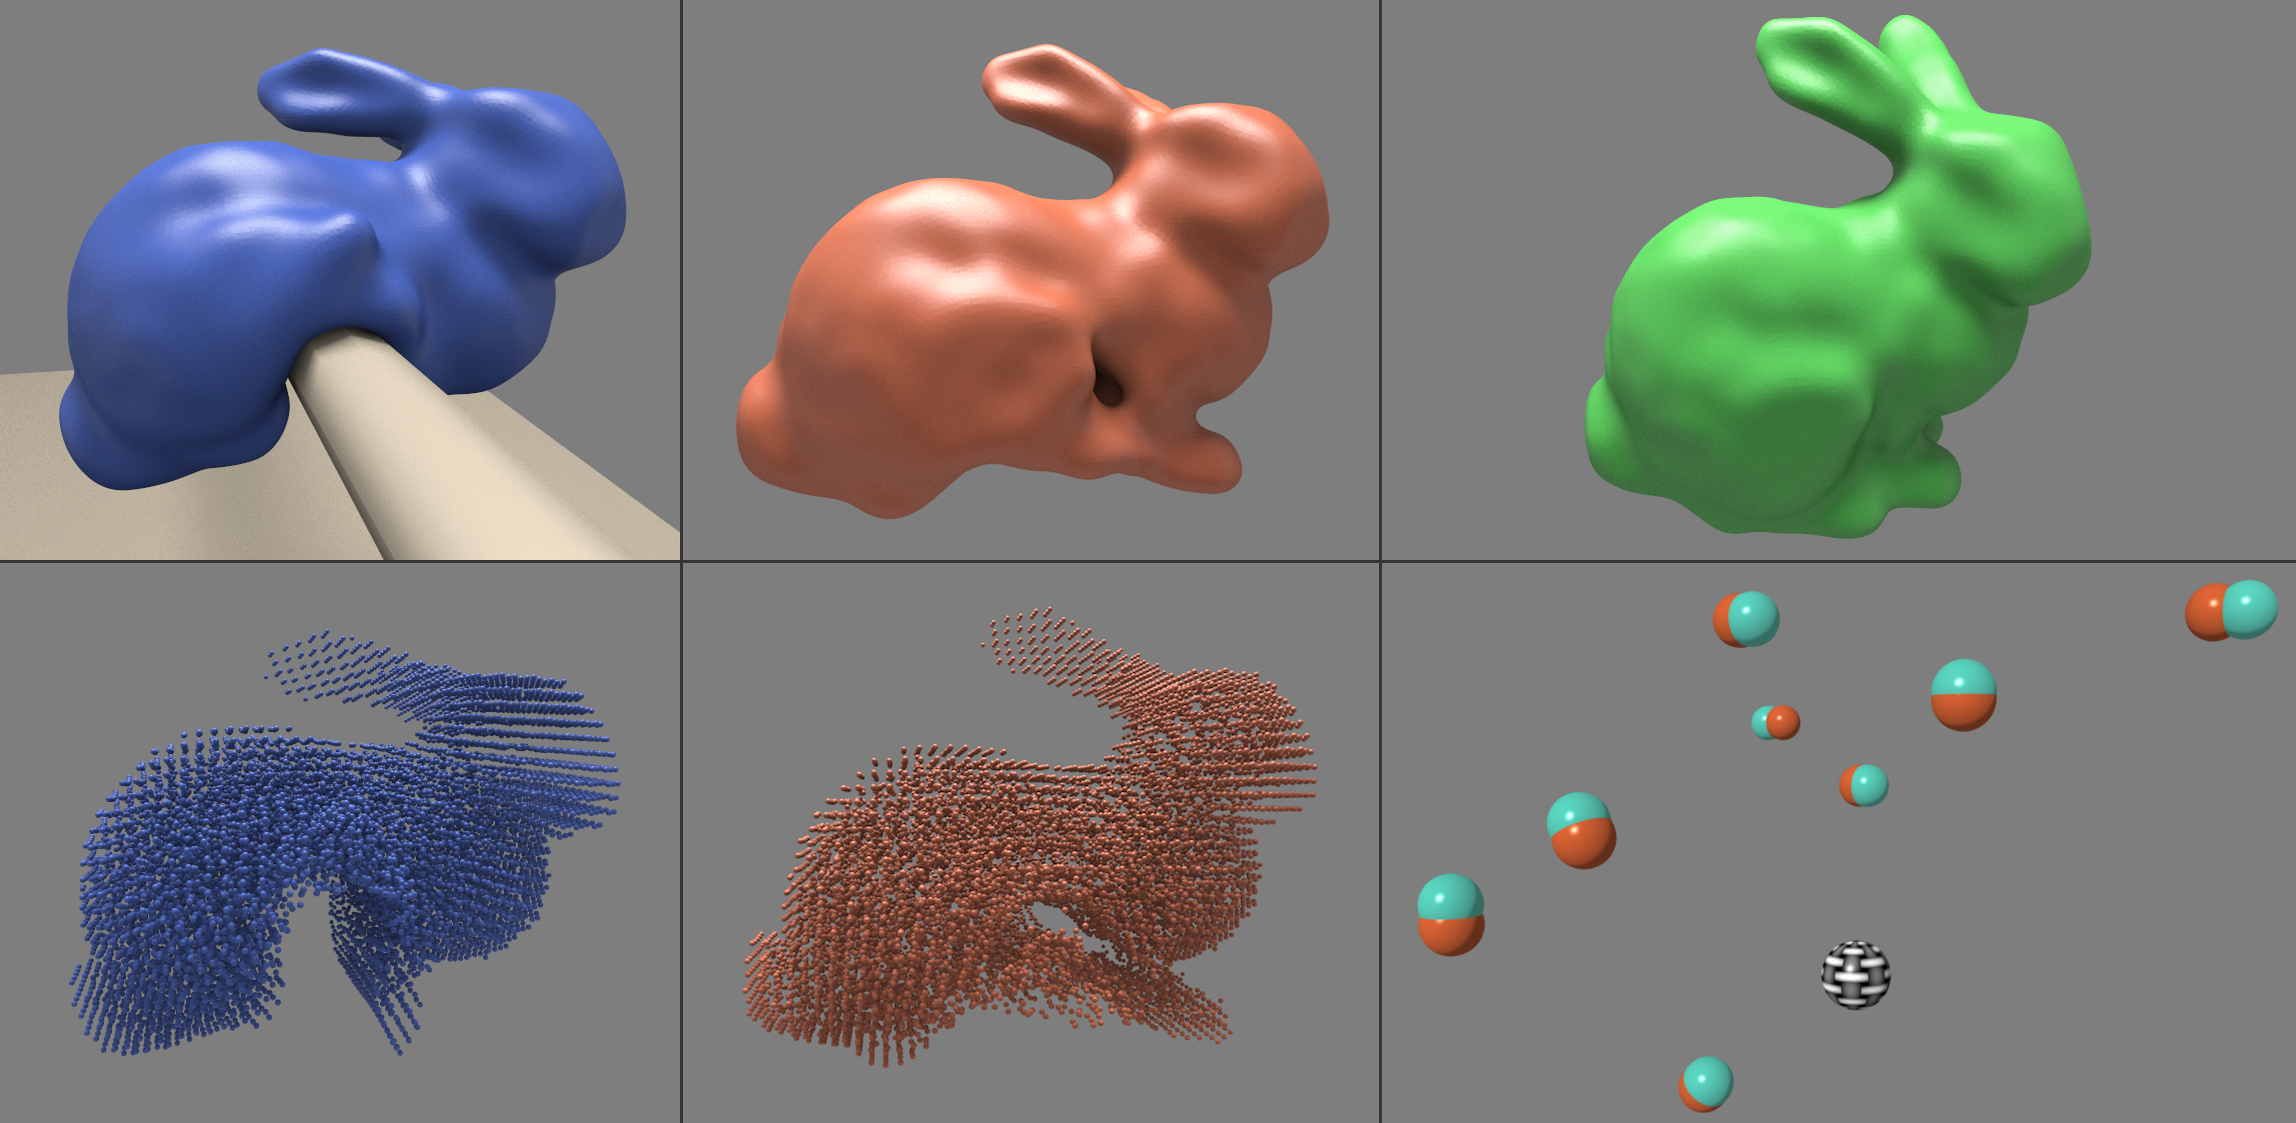
\includegraphics[width=6.1in]{Figures/teaser.png}
\caption{Sample frames from a sequential, point-based elastoplastic simulator, which we hope to accelerate with a GPU implementation.}
\label{fig:teaser}
\end{centering}
}

\maketitle





\begin{abstract}
We present a straightforward, easy-to-implement, point-based approach
for animating elastoplastic materials.  The core idea of our approach
is the introduction of {\em embedded space}---the least-squares best
fit of the materials rest state into three dimensions.  Together with
{\em plastic offsets} that map embedded space to rest space, the
embedded space allows us to robustly estimate the deformation
gradient, compute elastic forces, and account for plastic flow.  We
additionally introduce an estimate for the volume of a particle,
opening the door for non-uniform sampling, and describe a technique to
increase the robustness of point-based elastic simulation.
Our approach can handle
arbitrarily large elastic deformations and extreme plastic
deformations.  Because the approach is point-based, there is no need
for complex remeshing---the corresponding operation is a simple
neighborhood query in embedded space. We demonstrate our approach on a variety of
examples that display a wide range of material behaviors.
\end{abstract}



\section{Introduction}

Hello
%\begin{CRcatlist}
  %\CRcat{I.3.7}{Computer Graphics}{Three-Dimensional Graphics and Realism}{Animation};
  %\CRcat{I.6.8}{Simulation and Modeling}{Types of Simulation}{Animation}.
%\end{CRcatlist}

%\keywordlist


%----------------------------------------------------------------------------
%----------------------------------------------------------------------------




%\let\ORIGCaption\caption
%\renewcommand{\caption}[1]{\vspace{-0.025in}\ORIGCaption{#1}}

%----------------------------------------------------------------------------
%----------------------------------------------------------------------------


%\bibliographystyle{acmsiggraph-awb}
%\bibliography{monalisa}

\end{document}

